\section{Deep Learning and Symbolic Music Generation}
Various approaches to symbolic music generation use deep learning. However, there are considerable differences in the implementation, such as choice of architecture and representation, that influence the model's capabilities, use case, and what aspects the user can control. The following table \ref{table:bigtable} summarizes these key characteristics across a selection of approaches that inspire our model. For a comprehensive survey of representation, tasks, and evaluation methods used in symbolic deep learning music generation see \cite{Ji_Yang_Luo_survey_symbolic_2024}.

\begin{table}[H]
    \centering
    \renewcommand{\arraystretch}{1.2} % Adjust row height
    \setlength{\tabcolsep}{3pt} % Adjust column spacing
    \scriptsize % Set smaller font size
    \begin{tabular}{|p{2.5cm}|p{1.8cm}|p{3cm}|p{1cm}|p{1cm}|p{3cm}|p{2.5cm}|}
        \hline
        \textbf{Name} & \textbf{Architecture} & \textbf{Control} & \textbf{TV} & \textbf{MI} & \textbf{Dataset} & \textbf{Representation} \\
        \hline
        FolkRNN 2015 \cite{Sturm_Ben-Tal_2016} & RNN & meter, mode & No & No & TheSession \cite{sessionfolkdata} & ABC\\
        DeepBach 2017 \cite{Hadjeres_Pachet_Nielsen_2017} & RNN & Inpainting & Yes & Yes & JSB-chorales \cite{jsbchorales} & Midi-Like\\ 
        MusicTransformer (2018) \cite{Huang_Vaswani_Uszkoreit_Shazeer_Simon_Hawthorne_Dai_Hoffman_Dinculescu_Eck_2018} & Transformer & - & No & No & Maestro \cite{hawthorne2018maestro},  JSB-chorales\cite{jsbchorales} & Midi-Like\\
        MuseNet 2019 \cite{Christine_2019} & Transformer & instrument, genre & Yes & Yes & Mastro \cite{hawthorne2018maestro}, CX \cite{classicalarchives}, BM \cite{bitmidi} & ?\\
        MidiNet 2019 \cite{midinet} & GAN & chords, melody & Yes & Yes & HTPM \cite{hooktheorypopmidi} & Midi-Like\\
        Fader Nets 2020\cite{Tan_Herremans_2020} & VAE & arousal & No & No & Maestro \cite{hawthorne2018maestro} & Custom \\
        MMM 2020 \cite{Ens_Pasquier_2020_MMM} & Transformer & inpainting, instrument, note-density & Yes & Yes & Lakh MIDI \cite{Raffel_2016} & MMM\\
        PopTransformer 2020 \cite{Huang_Yang_remi_pop_transformer_2020} & Transformer & chords, tempo & Yes & No & Custom & REMI\\
        Museformer 2022 \cite{Yu_Lu_Wang_Hu_Tan_Ye_Zhang_museformer_2022} & Transformer & - & No & Yes & LakhMIDI \cite{Raffel_2016} & REMI-Like\\
        Polyfussion 2023 \cite{Min_Jiang_Xia_Zhao_polyffusion_2023} & Diffusion & inpainting, texture & Yes & No & POP90 \cite{Wang_Chen_pop90_dataset} & Piano-Roll\\
        FIGARO 2023 \cite{Rütte_figaro_2023} & Transformer & chords, instrument, meter, note-density & Yes & Yes & Lakh MIDI \cite{Raffel_2016} & REMI+ \\
        MMT 2023 \cite{Dong_Chen_MMT_Kirkpatrick_2023} & Transformer & instrumentation & No & Yes & Lakh MIDI \cite{Raffel_2016}, SOD \cite{Crestel_OrchestralDataset} & Midi-Tuple \\
        Sympack 2024 \cite{Chen_Smith_Spijkervet_Wang_Zou_Li_Kong_Du_2024} & Transformer & chords, structure, notes & Yes & Yes & Lakh MIDI\cite{Raffel_2016}, \cite{Bertin-Mahieux_Ellis_Whitman_Lamere_2011}, Custom & -\\
        Tunesformer 2023 \cite{tunesformer} & Transformer & Form & Yes & No & IrishMAN\cite{tunesformer} & ABC \\
        MuseCoco 2023 \cite{Lu_Xu_Kang_Yu_Xing_Tan_Bian_MuseCoco_2023} & Transformer & Genre, tempo, emotion ...  & No & No & Custom & REMI-Like\\
        MuseBarControl 2024 \cite{Shu_Xu_Musebarcontrol_2024} & Transformer & chords & Yes & No & POP90 \cite{Wang_Chen_pop90_dataset} & REMI-Like\\
        NTT 2024 \cite{Ryu_Dong_nested_2024} & Transformer & - & No  & Yes & Lakh MIDI \cite{Raffel_2016}, POP90 \cite{Wang_Chen_pop90_dataset}, SOD \cite{Crestel_OrchestralDataset} & Compound\\
        FTG 2024 \cite{Zhu_Liu_Jiang_Zheng_texture_2024} & Diffusion & texture, rhythm, chords & Yes & No & POP90 \cite{Wang_Chen_pop90_dataset} & Piano-Roll \\
        NDRD 2024 \cite{Huang_rule_diffusion_2024} & Diffusion & chord, pitch, note-density & Yes & No & Maestro \cite{hawthorne2018maestro}, POP90 \cite{Wang_Chen_pop90_dataset} & Piano-Roll \\
        NotaGen 2025 \cite{wang2025notagenadvancingmusicalitysymbolic} & Transformer & instrumentation, genre & No & Yes & Custom & ABC (interleaved)\\
        \hline
    \end{tabular}
    \caption{Overview of symbolic, deep learning based music generation models, their architectures, and control mechanisms, time-vayring control (TV), multitrack capabilities (MI), dataset, and representation. A more complete Overview
    is found in \cite{Ji_Yang_Luo_survey_symbolic_2024}}
    \label{table:bigtable}
\end{table}

\section{Representation and Format}\label{section:representation}
The choice of representation of data is a crucial aspect of music generation. First, the choice of audio or symbolic music has consequences for data availability, dataset size, context of the output, and what features can be controlled. Second, tokenization, the method in which symbolic or audio data are chunked, organized, and ingested into the model is an important aspect, with tradeoffs to consider for different generative tasks and goals. 


\subsection{Symbolic Music vs Audio}\label{section:symbolic_audio}
Music can be represented digitally in two ways, either as an audio rendition or symbolically as a set of instructions. Working with different representations comes with various drawbacks and benefits for music generation. There are different types of symbolic representations of music, but the most common consists of discrete sequences of musical elements such as pitch or duration.  Working with audio theoretically gives access to all audible qualities of music, including detailed information on instrumental timbre or acoustic settings. In symbolic music, this is more restricted. 

Symbolic data is also far less available than audio data. Many symbolic music datasets are created by compiling hand-transcribed music. High-quality automatic transcription from audio remains an unsolved issue.\cite{Ji_Yang_Luo_survey_symbolic_2024}\cite{Chen_Smith_Spijkervet_Wang_Zou_Li_Kong_Du_2024}. This is a serious limiting factor on how large symbolic music generators can become. However, symbolic music gives more direct access to many higher-level musical features such as chord progressions, melodies, and instrumentation. When working with audio, these features have to be extracted first, requiring additional processing steps that are prone to inaccuracies. 
Another consideration to account for is size: raw audio is significantly larger than corresponding symbolic music. In addition, rendered audio is difficult to edit once generated. 
 
\subsection{Tokenisation}\label{section:tokenization}
Sequences are typically transformed into tokens, a numerical representation of data, to be handled by a machine learning algorithm. Audio-based music generation uses tokenization to condense audio while retaining its semantic content. Jukebox \cite{Dhariwal_Jun_Payne_Kim_Radford_Sutskever_2020} uses a variational autoencoder\cite{Kingma_Welling_2014} with a discretizing bottleneck (VQ-VAE) to create tokens from audio. Musicgen \cite{copet2023simple} tokenizes audio using the previously developed Encodec model for audio compression which, similarly to VQ-VAE, learns a highly condensed discrete representation of audio \cite{Défossez_2023_encodec}. These condensed encodings are crucial for generative modeling on audio. Depending on the representation, a similar technique is used to encode piano rolls for diffusion of symbolic music \cite{Min_Jiang_Xia_Zhao_polyffusion_2023}\cite{Zhu_Liu_Jiang_Zheng_texture_2024}.

\subsection{Symbolic Tokenisation} \label{section:symbolic_tok}
Symbolic music is represented is in different ways, such as text (i.e. the ABC notation), piano roll, graph, and sequences. The most widely used representation, however, is the event-based MIDI representation. Which is reflected in the tokenization techniques. In symbolic music, tokenizers are feature extractors. They extend the standard MIDI vocabulary with additional tokens that help models better capture different aspects of music.\cite{Fradet_Briot_Chhel_2021}. In table \ref{table:bigtable} the tokenization approach of different symbolic models is summarized. \textbf{MIDI-Like} tokenization closely emulates the MIDI vocabulary, translating a MIDI file into a single stream of tokens such as note-on and note-off. The \textbf{MMM} tokenizer adds indicators to aid track-inpainting. \textbf{REMI} \cite{Huang_Yang_remi_pop_transformer_2020} tokenization expands on MIDI-based tokenization with tokens for duration, bar, and position, designed to help capture recurring musical patterns. \textbf{REMI+} \cite{Rütte_figaro_2023} tokenization extends \textbf{REMI} with an instrument token to better encode multi-instrument tracks. The \textbf{PerTok} tokenizer designed by Lemonaid\footnote{https://www.lemonaide.ai/}  encodes micro timings and offsets designed to capture the full spectrum of rhythm in musical performances.\\

These extensions come at a cost: The resulting sequences of tokens can become very long, which adversely affects the model \cite{Ji_Yang_Luo_survey_symbolic_2024}. Ongoing attempts such as compound word or nested tokens aim to shorten the sequences by combining low-level tokens into more expressive high-level tokens.\cite{Ryu_Dong_nested_2024}. Dong et al. \cite{Dong_Chen_MMT_Kirkpatrick_2023} combine six different MIDI-like events (type, beat, position, pitch, duration, instrument) into single tokens. Hsiao et al. \cite{compound_word_Hsiao_Liu_Yeh_Yang_2021} differentiate between token types and group neighboring tokens into compound words, resulting in significantly shorter sequences (about 50\% compared to individual tokens). 

This thesis uses a third approach: Byte Pair Encoding (BPE) \cite{Sennrich_Haddow_Birch_BPE_2016}. BPE is a bottom up tokenisation approach, used widely in language modeling, including the GPT series of models \cite{Radford_Wu_Child_Luan_gpt2_2019}\cite{jurafskybook} and has been successfully applied to symbolic music generation \cite{Fradet_Gutowski_Chhel_Briot_2023}. The approach is simple: the most common token pairs of the dataset are repeatedly combined into new combined tokens until the total amount of unique tokens reaches a preset vocabulary size. This approach works independently of token types and semantic content of the tokens and allows for very flexible scaling of the vocabulary. As seen in figure \ref{fig:tok_compare}, this drastically shortens the sequence length by about a third ($mean_{individual}=47976, mean_{bpe}=14519$), which in turn improves both the quality and efficiency of the model. 


\begin{figure}[H]
    \centering
    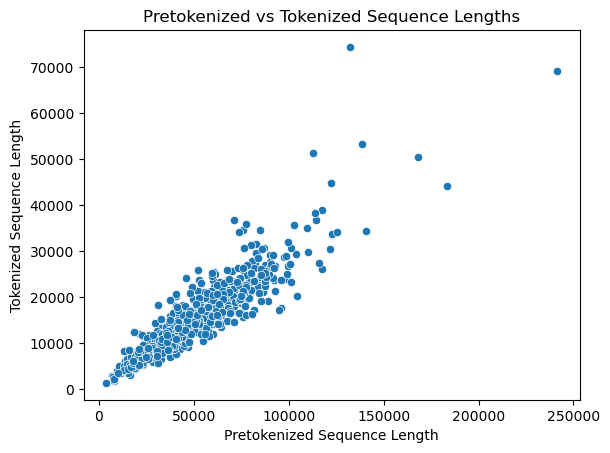
\includegraphics[width=0.5\textwidth]{IMAGES/scatter_pre_post_tok.png} 
    \caption{Scatterplot of sequence length before and after BPE tokenisation}
    \label{fig:tok_compare}
\end{figure}
\section{Control} \label{section:control}
Control is an essential aspect of any generative model. Without control, even the best generative models producing beautiful music are of limited real-world use. Control allows generative AI tools to become proper collaborative systems, which generate for a wide array of scenarios. In music generation, control covers essentially all musical features. Available features vary by representation. To illustrate:
Raw audio models such as Stable Audio (Evans et al., 2024) can be controlled for acoustic settings (i.e jazz music playing in a \textit{busy restaurant}, in a \textit{large cathedral}, or \textit{through an intercom}), something that is simply not represented in symbolic music. 

There are different approaches to classifying musical features. 
One can differentiate between global and local features \cite{Van_Kranenburg_Volk_Wiering_2013} (discussed in the appendix \ref{feature_cat}), 
deep vs surface-level features \cite{Blacking_1971}, high-level versuss low-level features \cite{Tan_Herremans_2020} and global versus fine-grained or time-varying features. 

In the context of this thesis, we differentiate between global features and time-varying features \cite{Rütte_figaro_2023}. Global features as features that do not change within an excerpt, while time-varying features can change within an excerpt. What is time-varying or global is highly context-dependent, a piece may have a single time time-signature and tempo as is assumed in \cite{Lu_Xu_Kang_Yu_Xing_Tan_Bian_MuseCoco_2023} or it may vary throughout the piece as enabled in \cite{Rütte_figaro_2023} or \cite{Huang_Yang_remi_pop_transformer_2020}. Other time varying controls could be chords \cite{Rütte_figaro_2023}\cite{Wu_Donahue_musicontrolnet_2023}\cite{Lan_Hsiao_Cheng_Yang_musicongen_2024}\cite{Min_Jiang_Xia_Zhao_polyffusion_2023}, melody \cite{copet2023simple}\cite{Min_Jiang_Xia_Zhao_polyffusion_2023} or texture \cite{Min_Jiang_Xia_Zhao_polyffusion_2023}. For the target application in a MACT - game, time-varying controls are necessary to provide a change in music that triggers a change in the patient's improvisation. See table \ref{table:bigtable} for an overview of what features are controlled for in recent deep learning symbolic music generators, and whether they are time varying or not. 
 

\subsection{Rhythmic control} \label{section:rhytmic_weight}
The types of control exercised over rhythmic components and rhythmic structure vary by representation as discussed in \ref{section:representation}. In CocoMulla \cite{Lin_cocomulla_2024} generated audio is controlled with drum tracks and a piano roll. Similarly, in JASCO\cite{Tal_jasco} drum audio is used for conditioning. In MusicConGen \cite{Lan_Hsiao_Cheng_Yang_musicongen_2024}, control for rhythm is added through tracking beats and downbeat. MusicControlNet \cite{Wu_Donahue_musicontrolnet_2023} adds beat and downbeat conditioning to an audio diffusion model.
For symbolic systems, control of tempo and meter is relatively common \cite{Rütte_figaro_2023}, \cite{Huang_Yang_remi_pop_transformer_2020}, \cite{Lu_Xu_Kang_Yu_Xing_Tan_Bian_MuseCoco_2023}. Time-varying control over rhythm is often deployed through note density (both vertical and horizontal)\cite{Rütte_figaro_2023}\cite{Huang_rule_diffusion_2024}. Another approach \cite{Zhu_Liu_Jiang_Zheng_texture_2024} involves passing the piano roll as a factor to guide the diffusion process. In Polyffusion \cite{Min_Jiang_Xia_Zhao_polyffusion_2023} Min et al. successfully encode texture that is disentangled into harmony and rhythm using a pre-trained variational auto-encoder \cite{Wang_vae_chord_rhythm_2020}. Herremans et al. \cite{Tan_Herremans_2020} control rhythm through the high-level feature arousal, which they disentangle into rhythm and note density using a variational auto-encoder. 

\subsection{Inner Metric Analysis} \label{section:ima}
We investigate Inner Metric Analysis (IMA) for its potential to control the rhythm structure of a generated excerpt over time. Unlike feature disentanglement discussed in section \ref{section:rhytmic_weight}, IMA is relatively simple algorithmic process that does not require any training. IMA has been used in the classification of dance-music \cite{Chew_Volk_Lee_Dance_metric_weight_2005}, automatic detection of meter \cite{Haas_Volk_2016} and music retrieval \cite{Volk_Garbers_VanKranenburg_Wiering_Grijp_Veltkamp_2009} as well as the study of syncopation \cite{Bemman2024}\cite{Volk2008Syncopation}.
Inner Metric Analysis identifies strong and weak pulses and their periods within note onsets in symbolic music. It is used to identify \textit{local meters} as opposed to \textit{outer meter} given by time-signatures.

A local meter is a set of evenly spaced onsets with a minimum length of three, not able to be extended forward or backward in time, and not contained within any other local meter. (see figure \ref{fig:ima_all}). Let $M(l)$ be the set of local meters with a length of at least l. The parameter $p$ is variable and determines how much the length of a local meter influences its weight. Intuitively, longer and more established local meters should carry more weight. This is given by $k_{m}^p$. The weight of an onset $W_{l,p}(o)$ is defined as the weighted sum of the local meters.  
The metric weight is calculated as follows \cite{Volk2008Syncopation}.  

\begin{equation}
 W_{l,p}(o) = \sum_{m \in M(l):o \in m}k_{m}^{p}
\end{equation} 
Spectral weight is a variation of metric weight, that considers the extension of each local meter: $ext(m)$. The red triangles in figure \ref{fig:ima_all} are an example of extensions. The calculation is similar, but it assigns a weight to each time point (instead of only to onsets) and considers the extensions. This feature is less sensitive to local changes.

\begin{equation}
 SW_{l,p}(t) = \sum_{m \in M(l):t \in ext(m)}k_{m}^{p}
\end{equation}

IMA can indicate rhythmic complexity. This, in turn, influences the ease of tapping along/following \cite{Volk2008Syncopation} and rhythmic entrainment. Configured properly, IMA could be utilized to control a music generator, steering the generated music so that it is more or less difficult to follow, allowing for difficulty adjustment in the context of a MACT game. 


\begin{figure}[H]
    \centering
    \begin{subfigure}{0.45\textwidth}
        \centering
        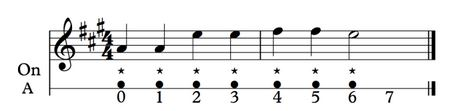
\includegraphics[width=\linewidth]{IMAGES/IMA1.JPG}
        \caption{Single local meter and its pulses (A) from the melody "Twinkle, Twinkle Little Star"}
        \label{fig:ima1}
    \end{subfigure}
    \begin{subfigure}{0.45\textwidth}
        \centering
        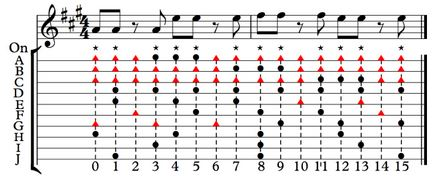
\includegraphics[width=\linewidth]{IMAGES/IMA2.JPG}
        \caption{10 local meters and their pulses produced by IMA of a syncopated variation of "Twinkle, Twinkle Little Star"}
        \label{fig:ima2}
    \end{subfigure}
    
    \vspace{0.5cm} % Adjust spacing between rows

    \begin{subfigure}{0.45\textwidth}
        \centering
        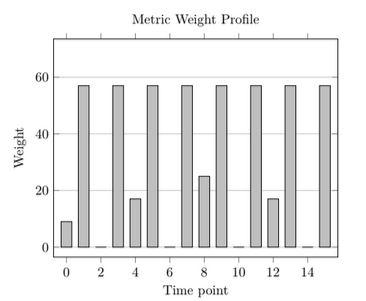
\includegraphics[width=\linewidth]{IMAGES/IMA3.JPG}
        \caption{Metric weight profile of syncopated "Twinkle, Twinkle Little Star"}
        \label{fig:ima3}
    \end{subfigure}
    \begin{subfigure}{0.45\textwidth}
        \centering
        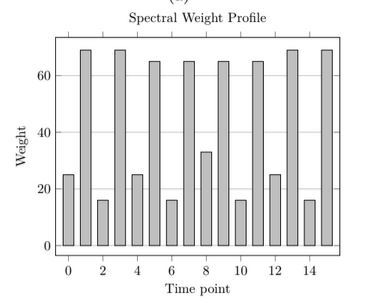
\includegraphics[width=\linewidth]{IMAGES/IMA4.JPG}
        \caption{Spectral weight profile of syncopated "Twinkle, Twinkle Little Star"}
        \label{fig:ima4}
    \end{subfigure}

    \caption{Visualisation of metric weight analysis \cite{Bemman2024}}
    \label{fig:ima_all}
\end{figure}

\section{Implementation of control} \label{section:addingcontrol}
Methods of enabling control in generative models can be split into four approaches. 1: Choice of architecture, 2: training data, 3: fine-tuning, and 4: post-hoc guidance. In table \ref{table:bigtable} we list a selection of recent symbolic deep-learning music generators with their corresponding architectures and datasets. Since deep learning models are often probabilistic, the control mechanisms are as well. They do not guarantee that the output has certain characteristics, but they \textit{condition} the probabilities of the outputs so that the outputs are more likely to have certain characteristics. 

\subsection{Control through architecture}
The choice of architecture lends itself to different types of control/conditioning. Transformers are the next-token predictors that predict based on the prior sequence. The default training paradigm allows for control with a user-defined sequence. This is true for both audio-based models such as MusicGen \cite{copet2023simple}, Jukebox \cite{Dhariwal_Jun_Payne_Kim_Radford_Sutskever_2020} and MusicLM \cite{Agostinelli_Denk_Borsos_Engel_Verzetti_Caillon_Huang_Jansen_Roberts_Tagliasacchi_et_al._2023} as well as symbolic music models such as MMT \cite{Dong_Chen_MMT_Kirkpatrick_2023}, MusicTransformer \cite{Huang_Vaswani_Uszkoreit_Shazeer_Simon_Hawthorne_Dai_Hoffman_Dinculescu_Eck_2018} and MusicBERT \cite{Zeng_Tan_Wang_MUSICBERT_2021}. Diffusion models are quite flexible compared to transformers. One can use the same model for inpainting, continuation, and - depending on the representation - melody and accompaniment generation through masking \cite{Min_Jiang_Xia_Zhao_polyffusion_2023}\cite{Rombach_Blattmann_Lorenz_Esser_Ommer_2022}Transformers, on the other hand, have to be explicitly trained for these tasks. 

\subsection{Control through training data}
Joint training of a model with the desired control is the most common and robust method of enabling control in a generative model. MusicGen\cite{copet2023simple}, a recent text-to-music (audio) transformer is trained on 20000 hours of licensed music from Shutterstock and pond5 \footnote{https://www.shutterstock.com/music and https://www.pond5.com/} which includes textual descriptions and tags for genre, tempo, and other factors such as instrumentation. Control is achieved through the joint training of a text description and music. An example description is provided below: 

\textit{Inspirational dramatic background music! Perfect for trailer, background, advertising, historical film, movie about superheroes, teaser and many other projects!}\footnote{ https://www.pond5.com/royalty-free-music/item/95908062-inspiring-dramatic-epic-background-cinematic-music
}

Text-based control, while user-friendly and accessible to non-musicians, is inherently vague. Levels of detail and choice of words vary widely by dataset, even with standardized tags included, such as genre and tempo. This is also true of specialized music-text datasets such as MusicCaps \cite{Agostinelli_Denk_Borsos_Engel_Verzetti_Caillon_Huang_Jansen_Roberts_Tagliasacchi_et_al._2023}\cite{Lee_Doh_Jeong_2023_subjectivity_musiccaps}. For this reason, the creators of MusicGen \cite{copet2023simple} add melody conditioning alongside text conditioning and train their model jointly with the chromagram of the melody alongside the text. 

In MusicGenStyle \cite{Rouard_Adi_Copet_Roebel_Défossez_musicgenstyle_2024} the authors utilize classifier-free guidance to add style conditioning to MusicGen. They train a music-style encoder that transforms a random subsample of a given reference audio track into style tokens. The style tokens are combined with the embeddings of the text description and provided as prefixes to the model. The conditioner and the MusicGen transformer are trained jointly on the entire dataset. 
The creators of FIGARO \cite{Rütte_figaro_2023} enable time-varying control over instrumentation, note density, average pitch, and volume on a bar-by-bar level, in a symbolic music generator through joint conditioning of music and the selection of desired features while training. 
\subsection{Adding control through fine-tuning}

Both the melody conditioning of MusicGen \cite{copet2023simple} and the style conditioning of MusicGenStyle \cite{Rouard_Adi_Copet_Roebel_Défossez_musicgenstyle_2024} retrain the full MusicGen model on the entire dataset which comes at considerable cost. Fine-tuning or transfer learning is another method through which models are (re)-trained, but at a considerably smaller cost and using less data. Fine-tuning is widely used in the language domain to adjust large language models for niche use cases where the available data may not be sufficient to train a large model from scratch. In the examples of MusicGen and MusicGenStyle, the availability of data was not a limiting factor. The controlling elements, melody, and style, are inferred from the training data. However, fine-tuning may achieve additional control at a lower cost. 

MusiConGen \cite{Lan_Hsiao_Cheng_Yang_musicongen_2024} is a fine-tuned variation of MusicGen, which adds control for rhythm and chords. They propose the jump-finetuning mechanism a form of selective fine-tuning, where the original model, with 1.5 Billion parameters and 48 self-attention layers, is split into blocks consisting of 4 self-attention layers. They train the first layer of each block, freezing the remaining layers. Additionally, they apply adaptive in-attention to the first nine blocks: The output of a transformer layer is augmented with copies of the original condition. As a result, only a quarter of the original parameters are tunable, which enables training on consumer GPUs on just 250 hours of music sourced from YouTube (as opposed to 20000 hours).  In Coco-Mula \cite{Lin_cocomulla_2024}, the authors adjust a LLAMA adapter with just 4\% of parameters, keeping all original MusicGen parameters frozen and training only the adapter on a small dataset of 300 songs to add drum and chord conditioning. 

MuseBarControl \cite{Shu_Xu_Musebarcontrol_2024} is a fine-tuned version of MuseCoco \cite{Lu_Xu_Kang_Yu_Xing_Tan_Bian_MuseCoco_2023} which extends the global controls with time-varying bar level control for music-generation. They compare several approaches: In the first, they augment the prompt (which is generated from text) with additional tokens for bar-wise control of chords and adjust the loss function to incorporate that. In the second approach, they introduce two novel methods. First, they pre-adapt the new parameters (introduced by the Lora adapter) to a separate classification task, an auxiliary task. The model classifies whether the section of music corresponds with the control tokens. The classification head added to the model for this task is removed after training. In the third step, they introduce counterfactual loss to reinforce the model's attention to the control, by rewarding the difference in negative log-likelihood between an output with the original and an output with a changed attribute. They find that combining the three strategies, pre-adaptation on a separate task followed by counterfactual loss and prompt augmentation yields the strongest model. 

\subsection{Adding control through guidance}
Other methods do not involve any fine-tuning or retraining of the original model. Adding control with additional model inputs does require at least some amount of retraining, which is not always feasible, and adding many types of control may deteriorate the model's performance. In these cases, guidance can be used to steer the model towards a certain output.
In SMITIN \cite{Koo_Wichern_Germain_SMITIN_2024} the authors intervene at inference time, while the trained model is generating, to guide MusicGen\cite{copet2023simple}  towards a certain goal. They explore guidance for ensuring the presence of certain instruments (piano/drums/bass/guitar) and to increase the quality/realism of the generated audio. For this, the authors train linear probes that learn to associate the state of each transformer layer in the network with the goal (i.e. drums being present in the output). Depending on the output of the classification a term is added to each self-attention head, before the matrix projection stage of the self-attention calculation. Then the model is steered in the direction of the probe, which increases the probability of the desired quality (drums) being present in the generated music. For more details see the SMITIN \cite{Koo_Wichern_Germain_SMITIN_2024} and the attention calculation of Musicgen \cite{copet2023simple}. Guidance of transformer models has been explored in other contexts \cite{language_guide_rutte_2024}, such as influencing truthfulness, humor, and appropriateness in language generation models, with mixed results. 

In Diffusion models, the output is sampled over several steps. At each of these steps, it is possible to intervene with guidance to direct the sampling towards a specified goal. Huang et al. \cite{Huang_rule_diffusion_2024}, repeat each sampling stage several times, and choose the output that follows a set of rules most closely. ControlNet \cite{Zhang_Rao_Agrawala_2023} adds spatial control to image generators, allowing the guidance of image generation using sketches, poses, edges, and depth maps without retraining. MusicControlNet \cite{Wu_Donahue_musicontrolnet_2023} adapts this approach to music generation, adding control for time-varying features, such as melody, dynamics, and rhythm. 

\section{Evaluation} \label{section:evaluation}
How to evaluate generated music is still an open research question. There are no generally approved methods of establishing the quality of generated music.\cite{Yin_Reuben_Stepney_Collins_2023}. However, there are several common frameworks used to evaluate music. Music generation literature often distinguishes between objective and subjective evaluation. Despite what the name suggests, objective evaluation of generated music does not measure the aesthetic quality or beauty of the music objectivly. Instead, it encompasses automated, statistical methods of analyzing and comparing generated music to human-composed music. Subjective evaluation encompasses evaluation methods that center human judgment. 

\subsection{Subjective Evaluation}
For subjective approaches, the methods vary widely \cite{Xiong_Wang_ai_eval_methods_2023}. There are simple Turing-type tests that examine whether human listeners can distinguish between generated and human-written music. There are tournament-style surveys, where different musical pieces obtained by different methods (human-written vs computer-generated) compete against each other. The listeners repeatedly select their preferred piece \cite{Huang_Vaswani_Uszkoreit_Shazeer_Simon_Hawthorne_Dai_Hoffman_Dinculescu_Eck_2018}\cite{Rütte_figaro_2023}.
Another typical approach is using (Likert) ratings along different dimensions to separate different qualities of the music. \cite{Dong_Chen_MMT_Kirkpatrick_2023}, \cite{Yu_Lu_Wang_Hu_Tan_Ye_Zhang_museformer_2022} and \cite{Chen_Smith_Spijkervet_Wang_Zou_Li_Kong_Du_2024} collect Likert ratings on coherence, richness, arrangement and consistency. In \cite{Dong_Chen_MMT_Kirkpatrick_2023}, this takes the following form: \\
Coherence: Is [the music] temporally coherent? Is the rhythm steady? Are there many out-of-context notes?;
Richness: Is [the music] rich and diverse in musical textures? Are there any repetitions and variations? Is [the music] too boring?; 
Arrangement: Are the instruments used reasonably? Are the instruments arranged properly?; \\
The specific questions asked vary with the aims of the project: 
In \cite{Yin_Reuben_Stepney_Collins_2023}, Likert ratings are collected along the dimensions of stylistic success, aesthetic pleasure, repetition, melody, harmony, and rhythm. Here, the questions for stylistic success are relevant due to their use of generative models to produce music in a certain style, specifically classical string quartets, and classical piano improvisations. 
These evaluations are often paired with statistical hypothesis testing to investigate relationships between the various ratings of the model outputs. An example would be: \textit{There is no difference between ModelA and ModelB on ratings of stylistic success}. Or \textit{ratings of melodic success are positively correlated with ratings of aesthetic pleasure}.
Finally, there are expert evaluations (which can also include Likert ratings) but also detailed analyses or even performances of the produced music \cite{Sturm_Ben-Tal_2016} \cite{Yin_Reuben_Stepney_Collins_2023}. \\

\subsection{Objective Evaluation}

Objective evaluation of generated music includes model-specific metrics and different comparative statistical metrics evaluating the outputs in comparison to other data \cite{Xiong_Wang_ai_eval_methods_2023}. Model-specific metrics are generic evaluations of a model's success to approximate training data, these will vary depending on the model and are not indicative of stylistic success. Examples of this are Negative Log Likelihood \cite{Huang_Vaswani_Uszkoreit_Shazeer_Simon_Hawthorne_Dai_Hoffman_Dinculescu_Eck_2018} or Perplexity\cite{Rütte_figaro_2023}. 
More generally applicable are statistical investigations of the outputs, in comparison with other datasets. Measuring similarity in music is an ongoing field of research \cite{Gurjar_Moon_similarity_2018} for a large variefty of different use cases, such as music retrieval, cover, genre, and artist detection. A popular comparative metric is calculating the Kulback Leibler (KL) divergence between two datasets with respect to certain features, such as the count of intervals or unique pitch classes. However to obtain the KL divergence one has to select specific features that may only capture a subset of the desired properties. Similar issues arise with other distance metrics i.e. cosine similarity, earth movers distance, or maximum overlapping area. 

A popular method of evaluating the plausibility of generated data is using contrastive learning such as CLIP for images, CLAP for audio and \cite{Elizalde_Deshmukh_Ismail_Wang_2023} and CLAMP for symbolic music \cite{wu2024clamp2multimodalmusic}.  In contrastive learning representations from different modalities of the same piece, such as audio recordings, midi trasncriptions, sheet music or text are aligned in an embedding space. In training, contrastive models minimize the distance between matching attributes of different modalities. The resulting model can be used to evaluate how closely a piece of generated music matches a text prompt, or how similar two pieces of music are to each other. 

